% SOICT 2026 submission draft (v1) --- Springer LNCS format.
% Generated 2026-08-04 with the SNL paper-writing skill. FOR HUMAN REVIEW ONLY; not committed.
% Template: llncs.cls from https://soict.org/wp-content/uploads/2025/09/Latex-Template-for-Springer.zip
% NOTE: verify this llncs.cls/splncs04.bst pair against the official SOICT 2026 download before
% final submission. Bibliography entries marked [VERIFY] need bibliographic confirmation.
%
\documentclass[runningheads]{llncs}
%
\usepackage[T1]{fontenc}
\usepackage{graphicx}
\usepackage{amsmath}
\usepackage{booktabs}
\usepackage{tikz}
\usetikzlibrary{arrows.meta,positioning,fit,backgrounds}
%
% --- Canonical number macros (single source of truth; keeps sections consistent) ---
\newcommand{\qlikeHAR}{0.4603}
\newcommand{\qlikeNews}{0.4430}
\newcommand{\qliketstat}{-6.22}
\newcommand{\rmseHAR}{0.002923}
\newcommand{\rmseNews}{0.002734}
\newcommand{\rmsetstat}{-9.38}
\newcommand{\rsqHAR}{0.7749}
\newcommand{\rsqNews}{0.8031}
\newcommand{\diraccHAR}{48.47}
\newcommand{\diraccNews}{47.77}
\newcommand{\diracctstat}{-2.97}
\newcommand{\nseed}{3}
\newcommand{\ntick}{33}
%
\begin{document}
%
\title{A Per-Ticker News Gate Improves Volatility Magnitude Forecasts for VN30 Without Improving Direction}
%
\titlerunning{A Per-Ticker News Gate for VN30 Volatility Forecasting}
%
\author{Author One\inst{1} \and Author Two\inst{1}}
\authorrunning{Author One et al.}
%
\institute{VNUHCM University of Science, Ho Chi Minh City, Vietnam\\
\email{\{author1,author2\}@student.hcmus.edu.vn}}
%
\maketitle
%
\begin{abstract}
Volatility forecasts set risk limits and option prices for VN30, the most liquid stocks on
Vietnam's Ho Chi Minh Stock Exchange, yet price-only forecasters discard the Vietnamese-language news that
carries early information about volatility shocks. We augment a HAR-driven parallel LSTM--GAT
volatility backbone with a PhoBERT news branch and scale that branch per stock through a learned,
input-independent gate, so each ticker admits a different amount of news signal. Across three seeds
at a matched training budget, the gated news model lowers five-day-ahead test QLIKE from
\qlikeHAR{} to \qlikeNews{} (paired $t=\qliketstat$) and RMSE from \rmseHAR{} to \rmseNews{}
(paired $t=\rmsetstat$) against an identical HAR-only backbone, and both improvements pass a paired
$t$-test. Directional accuracy does not improve (\diraccHAR\% vs.\ \diraccNews\%, paired
$t=\diracctstat$, below the 5\% level). We show this is a property of the target rather than a model
defect: the day-to-day change in the single-day Parkinson volatility estimator is anti-persistent
(sign lag-1 autocorrelation $-0.30$, negative for all \ntick{} tickers), and model-free persistence
and trailing-mean forecasters reach the same $\approx 49\%$ ceiling while attaining negative
$R^2$. News therefore improves the forecast magnitude that the model can learn, and leaves
untouched a direction task that is near-random for every forecaster. We report the finding on a
Vietnamese emerging market where news-augmented volatility forecasting is largely unstudied.

\keywords{Volatility forecasting \and Graph neural networks \and Financial news \and PhoBERT \and
Emerging markets.}
\end{abstract}
%
% ======================================================================
\section{Introduction}
% Stakes: who suffers and why the domain matters.
Volatility forecasts drive the daily risk decisions of every desk that trades VN30, the basket of
roughly thirty most liquid stocks on Vietnam's Ho Chi Minh Stock Exchange. A margin engine sizes
collateral from forecast volatility; an option desk prices from it; a risk officer sets position
limits against it. When the forecast tracks tomorrow's realized volatility poorly, each of these
decisions pays for the error. VN30 desks make these decisions in an information environment that a
price-only forecaster ignores: a steady flow of Vietnamese-language news, from official press and
from brokerage research, that plausibly signals volatility shocks before they show up in the price
range.

% Problem gap: structural limitation of current approaches.
Two limitations keep existing forecasters from using that signal. First, the workhorse econometric
model, the Heterogeneous Autoregressive (HAR) model of Corsi~\cite{corsi2009}, is linear and
univariate: it regresses future volatility on its own daily, weekly, and monthly averages, with no
channel for text and no channel for cross-stock coupling. Second, the deep-learning forecasters
that add cross-stock structure through graph neural networks~\cite{velickovic2018,sonani2025}
remain price-only, and the smaller line of text-augmented work fuses a single market-wide sentiment
score by concatenation. Concatenation assumes every stock reads the same amount of information from
news. That assumption is wrong for VN30: a widely-covered bank and a thinly-covered utility do not
carry the same news intensity, and a model that admits news uniformly either starves the
well-covered names or injects noise into the quiet ones.

% Key abstraction.
We close both gaps with a \emph{per-ticker news gate}. A shared news branch encodes each stock's
daily news into a vector; a learned scalar per stock, passed through a sigmoid, then scales that
vector before it joins the price representation. The gate is a single number per ticker, learned by
gradient descent and independent of the day's input, so the model decides once, per stock, how much
of the news branch to admit. This turns "how much does news matter for this stock" from a modeling
assumption into a learned parameter.

% Design intuition.
The full model has two branches (Fig.~\ref{fig:arch}). A price branch reuses a fixed parallel
LSTM--GAT backbone: a per-stock long short-term memory (LSTM) network reads the three HAR
volatility scales over a 22-day window, and a graph attention network (GAT) mixes information
across stocks on a $k$-nearest-neighbour graph. A
news branch reads a 146-dimensional daily news vector per stock, built offline from PhoBERT
embeddings of Vietnamese articles, split into official-press and brokerage groups and carried
forward by an exponentially weighted average. The per-ticker gate scales the news branch, and a
final linear layer fuses the two branches into a five-day-ahead volatility forecast.

% Contributions.
This paper makes three contributions.
\begin{enumerate}
\item \textbf{Architecture.} We design a news-fusion volatility forecaster that gates a PhoBERT
dual-group news branch per stock and fuses it with a HAR-driven LSTM--GAT price backbone
(Section~\ref{sec:method}).
\item \textbf{News improves forecast magnitude.} Across three seeds at a matched 20-epoch budget,
the gated news model lowers five-day-ahead QLIKE from \qlikeHAR{} to \qlikeNews{} and RMSE from
\rmseHAR{} to \rmseNews{} against a HAR-only backbone; both pass a paired $t$-test
($t=\qliketstat$ and $t=\rmsetstat$, Section~\ref{sec:results}).
\item \textbf{Direction is near-random by construction.} We show that neither model improves
directional accuracy, and that the $\approx 48\%$ figure is the intrinsic ceiling of the task:
the daily Parkinson target's day-to-day change is anti-persistent, and model-free forecasters reach
the same ceiling (Section~\ref{sec:results} and Section~\ref{sec:discussion}).
\end{enumerate}

% Results preview.
On \ntick{} VN30 tickers over a temporal 70/15/15 split, the gated news model attains test
$R^2=\rsqNews$ against \rsqHAR{} for the HAR-only backbone, and the QLIKE and RMSE gains hold in the
same direction on all three seeds. The directional-accuracy result reframes a metric that earlier
drafts of this project reported as high (68--72\%) but which a measurement artifact had inflated;
the corrected figure is near coin-flip, and we explain it as a property of the data
(Section~\ref{sec:discussion}).

% ======================================================================
\section{Background and Problem Setup}
\label{sec:background}

\subsubsection{Parkinson volatility.}
We forecast daily volatility measured by the Parkinson range estimator, which uses the intraday
high $H$ and low $L$:
\begin{equation}
\sigma^2_{\text{Park}} = \frac{\left(\ln(H/L)\right)^2}{4\ln 2}.
\label{eq:parkinson}
\end{equation}
The range estimator uses more of the day's price path than a close-to-close estimator and is a
standard choice for daily data~\cite{parkinson1980}, and range-based inputs improve
realized-volatility forecasts within a HAR framework~\cite{korkusuz2023}. It is a noisy one-day
proxy for the latent volatility, a fact that Section~\ref{sec:discussion} shows matters for the
direction task.

\subsubsection{The HAR decomposition.}
The HAR model of Corsi~\cite{corsi2009} predicts future volatility from three moving averages of
past volatility, over a daily (1-day), weekly (5-day), and monthly (22-day) window. The three
scales approximate the long memory of volatility with a parsimonious linear regression. We use
these same three averages as the input features of the price branch, so the deep model starts from
the information HAR uses and adds temporal, cross-stock, and news structure on top.

\subsubsection{Forecast target and losses.}
For each stock and each day $t$ we predict the Parkinson volatility five trading days ahead, a
single-day value at $t+5$ (not a five-day average). We train with mean squared error on
normalized targets and evaluate on the original scale with the six metrics the project mandates:
MSE, RMSE, MAE, $R^2$, QLIKE, and directional accuracy. QLIKE, the quasi-likelihood loss standard
in the realized-volatility literature~\cite{patton2011}, penalizes under-prediction of volatility
more than over-prediction and tolerates the noise in the volatility proxy:
\begin{equation}
\text{QLIKE} = \frac{1}{T}\sum_{t=1}^{T}\left(\frac{\hat{\sigma}^2_t}{\sigma^2_t}
 - \ln\frac{\hat{\sigma}^2_t}{\sigma^2_t} - 1\right).
\label{eq:qlike}
\end{equation}
Directional accuracy measures how often the predicted change in volatility from one step to the
next matches the realized change in sign. We compute it \emph{per ticker over time}: for each
stock we compare $\operatorname{sign}(\hat{y}_{i,t+1}-\hat{y}_{i,t})$ against
$\operatorname{sign}(y_{i,t+1}-y_{i,t})$, then average across stocks. Section~\ref{sec:results}
explains why the naive alternative, which flattens all stocks and days into one array before taking
differences, reports a misleadingly high number.

% ======================================================================
\section{Method: Per-Ticker Gated News Fusion}
\label{sec:method}

The model reads two aligned inputs per 22-day window: a price tensor of HAR features and a news
tensor of PhoBERT-derived features, both indexed by stock and day. Two branches encode them
independently, a per-ticker gate scales the news branch, and a linear layer fuses the result into
one forecast per stock. Figure~\ref{fig:arch} shows the flow; we describe the price branch, the
news branch, the gate, and the fusion in turn.

\begin{figure}[t]
\centering
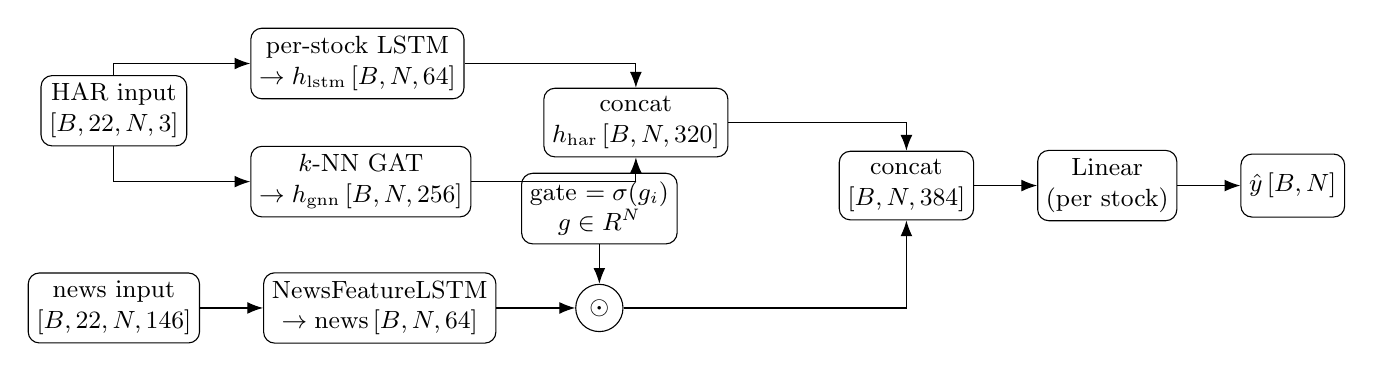
\begin{tikzpicture}[
  font=\small,
  box/.style={draw, rounded corners, align=center, minimum height=8mm, inner sep=3pt},
  op/.style={draw, circle, inner sep=1pt, minimum size=6mm},
  >={Latex[length=2mm]}
]
% price branch
\node[box] (harin) {HAR input\\ $[B,22,N,3]$};
\node[box, right=8mm of harin, yshift=6mm] (lstm) {per-stock LSTM\\ $\to h_{\text{lstm}}\,[B,N,64]$};
\node[box, right=8mm of harin, yshift=-9mm] (gat) {$k$-NN GAT\\ $\to h_{\text{gnn}}\,[B,N,256]$};
\node[box, right=10mm of lstm, yshift=-7.5mm] (harembed) {concat\\ $h_{\text{har}}\,[B,N,320]$};
% news branch
\node[box, below=16mm of harin] (newsin) {news input\\ $[B,22,N,146]$};
\node[box, right=8mm of newsin] (newslstm) {NewsFeatureLSTM\\ $\to \text{news}\,[B,N,64]$};
\node[op, right=10mm of newslstm] (mult) {$\odot$};
\node[box, above=5mm of mult] (gate) {gate $=\sigma(g_i)$\\ $g\in\mathbb{R}^{N}$};
% fusion
\node[box, right=14mm of harembed, yshift=-8mm] (concat) {concat\\ $[B,N,384]$};
\node[box, right=8mm of concat] (fuse) {Linear\\ (per stock)};
\node[box, right=8mm of fuse] (pred) {$\hat{y}\,[B,N]$};
% edges price
\draw[->] (harin) |- (lstm);
\draw[->] (harin) |- (gat);
\draw[->] (lstm) -| (harembed);
\draw[->] (gat) -| (harembed);
\draw[->] (harembed) -| (concat);
% edges news
\draw[->] (newsin) -- (newslstm);
\draw[->] (newslstm) -- (mult);
\draw[->] (gate) -- (mult);
\draw[->] (mult) -| (concat);
% fusion
\draw[->] (concat) -- (fuse);
\draw[->] (fuse) -- (pred);
\end{tikzpicture}
\caption{The per-ticker gated news-fusion model. The price branch (top) reuses a fixed parallel
LSTM--GAT backbone; the news branch (bottom) encodes PhoBERT features, which a learned gate
$\sigma(g_i)$ scales per stock before concatenation. $B$ is batch size, $N$ the number of stocks.}
\label{fig:arch}
\end{figure}

\subsection{Price branch: a fixed HAR LSTM--GAT backbone}
The price branch reuses, read-only, the parallel LSTM--GAT backbone of the project, adapted from the
hybrid LSTM--GNN design of Sonani et al.~\cite{sonani2025}. Its input is a tensor
$[B,22,N,3]$: a batch of $B$ windows, each covering 22 trading days for $N$ stocks with the three
HAR volatility scales. A per-stock LSTM (input size 3, hidden size 64, two layers, dropout 0.2)
encodes each stock's temporal path into $h_{\text{lstm}}\in\mathbb{R}^{B\times N\times 64}$. In
parallel, a two-layer graph attention network (four heads, hidden size 64) mixes information across
stocks on a $k$-nearest-neighbour graph built from return correlation, and a mean over the time
axis yields $h_{\text{gnn}}\in\mathbb{R}^{B\times N\times 256}$. Concatenating the two gives the
price representation $h_{\text{har}}\in\mathbb{R}^{B\times N\times 320}$. Used alone, with a dense
head, this backbone is the HAR-only baseline of Section~\ref{sec:results}; every news model reuses
its embeddings without changing a weight, so the comparison isolates the news contribution.

\subsection{News branch: dual-group PhoBERT features}
\label{sec:news}
The news branch consumes a 146-dimensional vector per stock per day, computed offline so that
training reads a cache rather than a language model. We build the vector in four steps.

\emph{Encode.} Each Vietnamese article (title and lead) passes once through
PhoBERT~\cite{phobert2020}, a BERT model~\cite{devlin2019} pre-trained on Vietnamese, yielding a
768-dimensional embedding cached by URL.

\emph{Attribute and reduce.} An article that names several stocks copies its embedding to each named
stock. Principal component analysis (PCA), fit only on data before the training cutoff to avoid
leakage, reduces each embedding to 32 dimensions.

\emph{Aggregate per stock-day.} When a stock has several articles on one day, we average their
32-dimensional vectors dimension by dimension into a single vector, and sum per-topic article counts
over seven topic categories (earnings, dividend, M\&A, management, regulation, macro, sector).

\emph{Split and carry forward.} We keep two source groups separately: an official-press group
(general news outlets) and a brokerage group (securities-firm research), so the model can weigh the
two differently. Because most days carry no fresh article for a given stock, we add an
exponentially weighted average of each group with a 30-trading-day half-life. On a day with no new
article the average decays by a factor $1-\alpha$ with $\alpha=1-\exp(-\ln 2/30)\approx 0.0228$;
on a day with an article it updates toward the new value. The half-life encodes the persistence of
a news effect: a report keeps some relevance for weeks rather than vanishing the next day. The 146
features are 32 embedding dimensions plus a norm for each of the two groups (66), the same for the
two exponentially weighted averages (66), and 14 topic counts.

A one-layer encoder maps this vector to a news representation. A linear layer
($146\to 64$) with a ReLU feeds a single-layer LSTM ($64\to 64$) over the 22-day window, producing
$\text{news}\in\mathbb{R}^{B\times N\times 64}$. The encoder processes each stock independently.

\subsection{The per-ticker gate}
\label{sec:gate}
A single scalar per stock controls how much news that stock admits. We hold a parameter vector
$g\in\mathbb{R}^{N}$, pass it through a sigmoid to get a gate in $(0,1)$ per stock, and scale the
news representation elementwise:
\begin{equation}
\text{news}^{\text{gated}}_{i} = \sigma(g_i)\cdot \text{news}_{i}, \qquad i=1,\dots,N.
\label{eq:gate}
\end{equation}
The gate does not depend on the day's input; it is one learned number per stock. Because the news
encoder processes stocks independently, the gate scales elementwise, and the fusion layer applies
per stock, the gradient of $g_i$ depends only on stock $i$'s own data. A unit test confirms this
isolation: changing another stock's label leaves $\partial\mathcal{L}/\partial g_i$ unchanged. We
give the gate its own optimizer group with a learning rate of 0.05, ten times the rate of the rest
of the network, so the gates move enough within the 20-epoch budget.

\subsection{Fusion}
Concatenating the price representation with the gated news representation gives
$[B,N,384]$, and a linear layer applied per stock produces the forecast
$\hat{y}\in\mathbb{R}^{B\times N}$, one five-day-ahead volatility value per stock per window. The
graph attention layer is the only place stocks exchange information, and it sits inside the price
branch, before the gate. From the gate onward the model treats stocks independently.

% ======================================================================
\section{Experimental Setup}
\label{sec:setup}

\subsubsection{Universe and split.}
We use \ntick{} VN30 constituents with daily open-high-low-close-volume (OHLCV) data. Series lengths range from about 1{,}300
sessions (SSB, listed 2021) to about 4{,}900 (VNM, ACB, from 2006). We exclude two current VN30
members, BSR and VPL, because their listing histories are too short to align with the panel: VPL
had 99 trading sessions and BSR 401 at data cutoff, and the graph model requires every stock to
have data on each shared date, so including VPL would shrink the common window to about 58 trading
days. We split each series chronologically into 70\% train, 15\% validation, and 15\% test to
prevent look-ahead leakage, and we fit all normalizers and the news PCA on the training portion
only.

\subsubsection{Training.}
We train for 20 epochs with the Adam optimizer~\cite{kingma2015}, a two-group learning rate (0.005
main, 0.05 gate), dropout 0.2, and early stopping on validation loss. We normalize HAR features and
targets with statistics from the training split and invert the transform before computing metrics
on the original volatility scale. To move from a single run to a comparison we can defend, we repeat
both the HAR-only backbone and the gated news model on three independent seeds (42, 123, 2026) at
this identical budget and report the mean, standard deviation, and a paired $t$-test across seeds.

\subsubsection{What the comparison controls.}
The two models share the price backbone, the data, the split, the seeds, the epoch budget, and the
batch configuration. They differ only in the news branch and its gate. A gain therefore attributes
to news fusion, not to a training-setup difference. We report results from the pipeline after two
corrections described in Section~\ref{sec:results}; earlier baselines in the project predate those
corrections and are not directly comparable, so we exclude them from the headline.

% ======================================================================
\section{Results}
\label{sec:results}

\subsection{News improves QLIKE and RMSE across seeds}
Table~\ref{tab:headline} reports the five-day-ahead test metrics for both models, averaged over
three seeds. The gated news model improves QLIKE from \qlikeHAR{} to \qlikeNews{} and RMSE from
\rmseHAR{} to \rmseNews{}. A paired $t$-test across the three seeds gives $t=\qliketstat$ for QLIKE
and $t=\rmsetstat$ for RMSE, both past the two-sided 5\% threshold for two degrees of freedom
($|t|>4.30$). The gains hold in the same direction on every seed: per-seed QLIKE differences are
$-0.0198$, $-0.0204$, and $-0.0118$, and per-seed RMSE differences are $-0.000183$, $-0.000228$,
and $-0.000159$. The model also raises $R^2$ from \rsqHAR{} to \rsqNews{} and lowers MAE from
$0.0008113$ to $0.0007930$.

\begin{table}[t]
\caption{Five-day-ahead test metrics, mean$\pm$std over three seeds (42, 123, 2026), 20 epochs
each. Lower is better for QLIKE, RMSE, MAE; higher for $R^2$; higher for directional accuracy
(DirAcc). The paired $t$ is across the three seeds; $|t|>4.30$ passes at the 5\% level with two
degrees of freedom.}
\label{tab:headline}
\centering
\begin{tabular}{lccc}
\toprule
Metric & HAR-only backbone & Gated news fusion & Paired $t$ (n=3) \\
\midrule
QLIKE            & $0.4603\pm0.0205$   & $\mathbf{0.4430\pm0.0185}$   & $-6.22$ (sig.) \\
RMSE             & $0.002923\pm0.000090$ & $\mathbf{0.002734\pm0.000096}$ & $-9.38$ (sig.) \\
MAE              & $0.0008113$         & $\mathbf{0.0007930}$         & n/a \\
$R^2$            & $0.7749\pm0.0140$   & $\mathbf{0.8031\pm0.0139}$   & n/a \\
DirAcc (\%)      & $\mathbf{48.47\pm0.35}$ & $47.77\pm0.52$           & $-2.97$ (n.s.) \\
\bottomrule
\end{tabular}
\end{table}

\smallskip
\noindent\textbf{Takeaway.} News fusion improves the metrics that score the forecast magnitude, and
the improvement survives a paired test across seeds rather than resting on one run. The gain is
modest in absolute terms (about 4\% of QLIKE) but consistent in sign.

\subsection{News does not improve direction}
Directional accuracy tells the opposite story. Both models sit near 48\%, below the 50\% no-skill
line, and the HAR-only backbone is nominally higher (\diraccHAR\% vs.\ \diraccNews\%). The per-seed
direction differences ($-0.53$, $-1.18$, $-0.42$ percentage points, all favouring HAR-only) give a
paired $t$ of $\diracctstat$, which does not pass the 5\% threshold. News neither helps nor
reliably hurts direction.

\subsection{A measurement correction behind these numbers}
Two corrections separate these numbers from earlier project reports. First, an earlier directional
accuracy of 68--72\% came from flattening predictions and targets into one $[\text{window},
\text{stock}]$ array before differencing, so most comparisons ran across different stocks on the
same day rather than the same stock across time. Same-day cross-stock comparisons benefit from
market-wide co-movement and inflate the score. The per-ticker metric of
Section~\ref{sec:background} removes this artifact and drops the figure to the intrinsic level.
Second, the backbone's feature normalizer had been fit but never applied, so earlier models trained
on raw, unnormalized volatility; applying it moved the headline QLIKE from about 0.55 to about
0.46. We report only post-correction numbers.

\subsection{Direction is near-random for every forecaster}
\label{sec:refbaselines}
To show the low directional accuracy is a property of the target rather than of the model, we run
two model-free reference forecasters against the identical per-ticker metric and target
construction. Table~\ref{tab:refs} gives the result. Persistence (predict the last observed
volatility) reaches 49.5\% direction, and a five-day trailing mean reaches 49.1\%, both
statistically indistinguishable from the trained models near 48\%. No forecaster, naive or trained,
beats coin-flip on this direction task. Yet the trained model's $R^2$ is strongly positive
($+0.76$ to $+0.79$) while both naive forecasters have \emph{negative} $R^2$, so the model does
real work on the volatility level while every forecaster fails on the day-to-day sign.

\begin{table}[t]
\caption{Directional accuracy and $R^2$ against the identical five-day target, per ticker,
averaged over \ntick{} tickers. The two reference forecasters use no learned parameters. The two
trained-model rows are the single reference run (seed 42) used for this like-for-like comparison;
their three-seed means (Table~\ref{tab:headline}) are 48.5\% and 47.8\% for direction and \rsqHAR{}
and \rsqNews{} for $R^2$, consistent within seed noise. Direction is near 49\% for all four; only
the trained models attain positive $R^2$.}
\label{tab:refs}
\centering
\begin{tabular}{lcc}
\toprule
Forecaster & Mean per-ticker DirAcc (\%) & Mean $R^2$ \\
\midrule
Persistence (last observed) & 49.5 & $-0.64$ \\
Trailing mean (5-day)       & 49.1 & $-0.08$ \\
HAR-only backbone (trained) & 48.1 & $+0.759$ \\
Gated news fusion (trained) & 47.6 & $+0.787$ \\
\bottomrule
\end{tabular}
\end{table}

\smallskip
\noindent\textbf{Takeaway.} The model forecasts the volatility level well and the day-to-day
direction no better than chance, because the direction of the daily target is close to
unpredictable for anyone. Section~\ref{sec:discussion} explains why.

% ======================================================================
\section{Discussion}
\label{sec:discussion}

\subsection{Why direction is near-random}
The forecast target is the single-day Parkinson estimator, and its day-to-day change is
anti-persistent. Measured on the full series of each stock, the sign of the daily change in
Parkinson volatility has a lag-1 autocorrelation of $-0.30$ on average, negative for all \ntick{}
tickers (range $-0.34$ to $-0.24$). An up-move in daily volatility tends to precede a
down-move: the estimator oscillates day to day around a slowly drifting level, a known property of
range-based daily volatility proxies. A forecaster that produces a smooth estimate of the level
cannot reproduce this high-frequency oscillation, so its directional calls decouple from the target
and sit at or just below 50\%. The per-ticker spread is tight (standard deviation about one
percentage point, 27 of \ntick{} tickers inside 48--52\%), so the near-random result is a shared
property of the universe rather than a few pathological stocks. News cannot rescue this direction
task because the task is near-random for structural reasons, and we base our conclusions on the
continuous-error metrics that reflect what the model can forecast.

\subsection{The gate improves accuracy but resists interpretation}
The per-ticker gate lowers aggregate QLIKE and RMSE, yet its learned values do not line up with
independent measures of which stocks should need news. Four methods (two feature-importance
analyses, an ablation on per-stock QLIKE change, and the learned gate itself) rank the stocks
differently, and we have no unified account of the disagreement. The gate earns its place as an
architectural mechanism that improves the aggregate forecast; it does not yet serve as a readout of
per-stock news relevance. We report this as an open question rather than claim an interpretation the
evidence does not support.

\subsection{A preliminary observation on forecast horizon}
An exploratory sweep over 1, 10, and 22-day horizons suggested that the news advantage concentrates
at short horizons and fades or reverses by 22 days, which a decay analysis would explain: the
30-day half-life news feature is nearly constant across these horizons, while volatility's own
predictability mean-reverts within days, so the room for a news increment shrinks as the horizon
grows. We flag this as preliminary only. The 1, 10, and 22-day runs predate the two corrections of
Section~\ref{sec:results} and have not been re-run on the corrected pipeline, so we do not state the
horizon reversal as a settled result. The structural evidence (news feature autocorrelation of 0.72
at 22 days versus volatility autocorrelation of 0.12) comes from raw data outside the training
pipeline, which the corrections do not touch, but the model comparison itself needs a
corrected, multi-seed re-run before we can cite it.

% ======================================================================
\section{Related Work}
\label{sec:related}

We place related work after the evaluation because the contribution is empirical: the value of the
per-ticker gate is visible only once the head-to-head numbers are on the table. Prior work falls
into three groups.

\subsubsection{Econometric volatility models.}
The HAR model~\cite{corsi2009} and its range-based inputs~\cite{parkinson1980} set the standard for
daily volatility forecasting and remain hard to beat. They are linear and univariate: no channel
admits text, and no channel couples one stock to another. We keep their multi-scale features as the
input of the price branch and add the structure they omit.

\subsubsection{Deep and graph-based forecasters.}
LSTM forecasters~\cite{hochreiter1997} capture nonlinear temporal structure, and graph attention
networks~\cite{velickovic2018} model cross-asset coupling; hybrid LSTM--GNN designs combine both for
stock prediction~\cite{sonani2025}. These forecasters remain price-only. Our price branch adopts the
hybrid LSTM--GNN backbone and adds a news branch that these designs lack.

\subsubsection{News- and text-augmented forecasting.}
Text-augmented forecasters add sentiment scores or news embeddings: an Attention-LSTM with a news
opinion index warns of systemic risk in China~\cite{ouyang2021}, and a growing line couples
sentiment analysis with graph neural networks for stock prediction~\cite{das2024}. These designs
usually fuse a single market-wide signal by concatenation, on English- or Chinese-language markets,
and concatenation admits the same amount of news to every asset. Our per-ticker gate replaces that
uniform admission with a learned per-stock scalar, and we work in Vietnamese with
PhoBERT~\cite{phobert2020} on VN30, an emerging market where news-augmented volatility forecasting
is little-studied. We do not compete on English benchmarks; we carve out the per-asset
news-relevance question that concatenation cannot express.

% ======================================================================
\section{Limitations and Conclusion}
\label{sec:conclusion}

\subsubsection{Limitations.}
Three limitations bound the claims. First, three seeds is the minimum for a paired $t$-test; five or
more would strengthen the QLIKE and RMSE result. Second, the \ntick{}-ticker universe differs
slightly from the official VN30 constituents (it keeps five long-history names that left the index
and excludes two short-history current members), so the dataset is a fixed, point-in-time VN30-like
universe rather than the live index. Third, the horizon observation of Section~\ref{sec:discussion}
is preliminary and needs a corrected re-run.

\subsubsection{Conclusion.}
A per-ticker news gate lets a HAR-driven LSTM--GAT volatility forecaster admit a different amount of
Vietnamese news for each VN30 stock, and it lowers five-day-ahead QLIKE and RMSE against a matched
price-only backbone with a paired $t$-test across seeds. The same model does not improve directional
accuracy, and we show that no forecaster does: the day-to-day direction of daily Parkinson
volatility is anti-persistent and near-random for structural reasons. News improves the volatility
magnitude a model can learn, and leaves untouched a direction task that the data itself makes
unlearnable. For a Vietnamese emerging market, this maps out both what news buys and what it cannot.

% NOTE FOR RIVF 2026 (secondary target, IEEE two-column, ~6 pages, EDAS): this LNCS draft needs a
% roughly 40--50% compression pass and a reformat to the IEEE class before that submission. Do not
% maintain two parallel documents; compress from this one when the RIVF timeline is confirmed.

%
% ---- Bibliography ----
% BibTeX users: \bibliographystyle{splncs04}. Entries below are hand-written for the draft; verify
% every [VERIFY] entry's exact venue/volume/pages/DOI before submission.
%
\begin{thebibliography}{99}

\bibitem{corsi2009}
Corsi, F.: A simple approximate long-memory model of realized volatility.
Journal of Financial Econometrics \textbf{7}(2), 174--196 (2009).
% [VERIFY] DOI 10.1093/jjfinec/nbp001 --- confirm volume/issue/pages.

\bibitem{parkinson1980}
Parkinson, M.: The extreme value method for estimating the variance of the rate of return.
The Journal of Business \textbf{53}(1), 61--65 (1980).
% [VERIFY] confirm volume/issue/pages.

\bibitem{patton2011}
Patton, A.J.: Volatility forecast comparison using imperfect volatility proxies.
Journal of Econometrics \textbf{160}(1), 246--256 (2011).
% [VERIFY] confirm as the QLIKE robust-loss reference; volume/pages.

\bibitem{hochreiter1997}
Hochreiter, S., Schmidhuber, J.: Long short-term memory.
Neural Computation \textbf{9}(8), 1735--1780 (1997).

\bibitem{velickovic2018}
Veli\v{c}kovi\'c, P., Cucurull, G., Casanova, A., Romero, A., Li\`o, P., Bengio, Y.:
Graph attention networks. In: International Conference on Learning Representations (ICLR) (2018).

\bibitem{devlin2019}
Devlin, J., Chang, M.-W., Lee, K., Toutanova, K.: BERT: Pre-training of deep bidirectional
transformers for language understanding. In: NAACL-HLT, pp. 4171--4186 (2019).

\bibitem{phobert2020}
Nguyen, D.Q., Nguyen, A.T.: PhoBERT: Pre-trained language models for Vietnamese.
In: Findings of the Association for Computational Linguistics: EMNLP 2020, pp. 1037--1042 (2020).
% [VERIFY] confirm page range.

\bibitem{kingma2015}
Kingma, D.P., Ba, J.: Adam: A method for stochastic optimization.
In: International Conference on Learning Representations (ICLR) (2015).

\bibitem{sonani2025}
Sonani, M.S., Badii, A., Moin, A.: Stock price prediction using a hybrid LSTM--GNN model:
integrating time-series and graph-based analysis. arXiv preprint arXiv:2502.15813 (2025).
% Verified against the source PDF (docs/paper/2502.15813v1.pdf): title, authors, arXiv id.

\bibitem{korkusuz2023}
Korkusuz, B., Kambouroudis, D., McMillan, D.G.: Do extreme range estimators improve realized
volatility forecasts? Evidence from G7 stock markets.
Finance Research Letters \textbf{55}, 103992 (2023).
% Verified against the source PDF (docs/paper/1-s2.0-S1544612323003641-main.pdf).

\bibitem{ouyang2021}
Ouyang, Z.-S., Yang, X.-T., Lai, Y.: Systemic financial risk early warning of financial market in
China using an Attention-LSTM model.
The North American Journal of Economics and Finance \textbf{56}, 101383 (2021).
% Verified against the source PDF (docs/paper/1-s2.0-S106294082100019X-main.pdf).

\bibitem{das2024}
Das, N., Sadhukhan, B., Chatterjee, R., Chakrabarti, S.: Integrating sentiment analysis with graph
neural networks for enhanced stock prediction: a comprehensive survey.
Decision Analytics Journal \textbf{10}, 100417 (2024).
% Verified against the source PDF (docs/paper/1-s2.0-S2772662224000213-main.pdf).

\end{thebibliography}
\end{document}
